%! Author = sriadityavedantam
%! Date = 4/8/26

\section{Bézout's Theorem}

\begin{definition}[Hypersurface]
    A hypersurface $H \subseteq \pp^n$ is a projective variety of the form
    \[
        H = \{F = 0\},
    \]
    where $F \in \c[x_0,\ldots,x_n]$ is homogeneous.
\end{definition}

\begin{theorem*}{
    Let $X \subset \pp^n$ be a smooth projective curve.
    Let $H \subset \pp^n$ be a hypersurface not containing $X$.
    Then
    \[
        X \cdot H = \deg(X)\deg(H).
    \]
}
\end{theorem*}

If $H = \{F = 0\}$, then $\deg(H) = \deg(F) = d$.

\begin{definition}[Hyperplane]
    A hyperplane $H' \subset \pp^n$ is a projective linear subspace of codimension $1$.
    If $H'$ intersects $X$ transversely, then
    \[
        \deg(X) = \#(X \cap H').
    \]
\end{definition}

\begin{definition}
    We say $X$ and $H'$ meet transversely at $P \in X \cap H'$ if
    \[
        T_P(X) + T_P(H') = T_P(\pp^n).
    \]
\end{definition}

\subsection*{Construction of the Intersection Divisor}

Since $F$ is not a global function on $\pp^n$, we work locally.

\textbf{(1)} Assume $X \not\subset \{x_i = 0\}$ for some $i$.
Otherwise, perform a projective change of coordinates.

\textbf{(2)} Let
\[
    U_i = \{x_i \neq 0\}, \quad \pp^n = \bigcup_{i=0}^n U_i.
\]
Define
\[
    f_i = \left.\frac{F}{x_i^d}\right|_{X \cap U_i}.
\]
Then $f_i$ is regular on $X \cap U_i$.

\textbf{(3)} The divisor $\div(f_i)$ on $X \cap U_i$ is effective and supported on
\[
    X \cap U_i \cap H.
\]
These local divisors glue to give a global divisor $\div(F)$ on $X$.

\begin{definition}[Intersection Number]
    The intersection number of $X$ and $H$ is
    \[
        X \cdot H \coloneqq \deg(\div(F)).
    \]
\end{definition}

\subsection*{Proof of Bézout's Theorem}

\begin{proof}
    Let $H = \{F = 0\}$ and $H' = \{F' = 0\}$ be hypersurfaces with $\deg(F) = \deg(F')$.
    Then $H \sim H'$.

    We claim
    \[
        X \cdot H = X \cdot H'.
    \]

    Observe
    \[
        \div(F) - \div(F') = \div\!\left(\frac{F}{F'}\right).
    \]
    Since $\deg(F) = \deg(F')$, we have
    \[
        \frac{F}{F'} \in \c(\pp^n),
        \quad
        \left.\frac{F}{F'}\right|_X \in \c(X).
    \]
    Thus $\div(F) \sim \div(F')$ on $X$.

    On a smooth projective curve, linearly equivalent divisors have the same degree.
    Hence
    \[
        X \cdot H = X \cdot H'.
    \]

    Now factor $F'$ into linear forms:
    \[
        F' = L_1 \cdots L_d.
    \]
    Then
    \[
        H' = H_1 \cup \cdots \cup H_d,
        \quad
        H_i = \{L_i = 0\}.
    \]

    Therefore
    \[
        X \cdot H'
        = \sum_{i=1}^{d} X \cdot H_i.
    \]

    Each $H_i$ is a hyperplane, so
    \[
        X \cdot H_i = \deg(X).
    \]

    Thus
    \[
        X \cdot H' = d \cdot \deg(X) = \deg(H)\deg(X).
    \]

    Hence
    \[
        X \cdot H = \deg(X)\deg(H).
    \]
\end{proof}

\subsection*{Examples}

\begin{figure}[H]
    \centering
    \captionsetup{justification=centering}

    \tikzset{every picture/.style={line width=0.75pt}}

    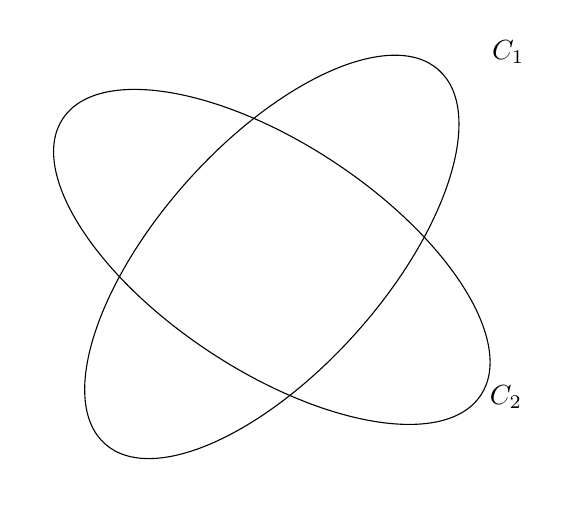
\begin{tikzpicture}[x=0.75pt,y=0.75pt,yscale=-1,xscale=1]
        \draw   (224.43,75.43) .. controls (241.08,50.25) and (299.67,59.64) .. (355.29,96.42) .. controls (410.91,133.19) and (442.5,183.41) .. (425.85,208.6) .. controls (409.2,233.78) and (350.62,224.39) .. (295,187.61) .. controls (239.38,150.84) and (207.78,100.62) .. (224.43,75.43) -- cycle ;
        \draw   (244.75,232.09) .. controls (222.23,211.98) and (239.96,155.36) .. (284.36,105.62) .. controls (328.76,55.87) and (383.01,31.84) .. (405.54,51.94) .. controls (428.06,72.05) and (410.32,128.67) .. (365.93,178.41) .. controls (321.53,228.16) and (267.27,252.19) .. (244.75,232.09) -- cycle ;

        \draw (439,43.4) node {$C_1$};
        \draw (438,209.4) node {$C_2$};
    \end{tikzpicture}

    \caption{Two curves intersecting in the expected number of points.}
\end{figure}

In general position, the number of intersection points equals $\deg(C_1)\deg(C_2)$.

\begin{figure}[H]
    \centering
    \captionsetup{justification=centering}

    \tikzset{every picture/.style={line width=0.75pt}}

    \begin{tikzpicture}[x=0.75pt,y=0.75pt,yscale=-1,xscale=1]
        \draw   (205,120) circle (69);
        \draw   (343,120) circle (69);

        \draw (184,40.4) node {$C_1$};
        \draw (412,41.4) node {$C_2$};
    \end{tikzpicture}

    \caption{Affine intersection vs. projective intersection.}
\end{figure}

Let $\pp^2_{[x,y,z]}$ with affine chart $z \neq 0$.
Then
\[
    C_1 : x^2 + y^2 = z^2,
    \quad
    C_2 : (x - z)^2 + y^2 = z^2.
\]

On the affine chart $z = 1$:
\[
    x^2 + y^2 = 1,
    \quad
    (x-1)^2 + y^2 = 1.
\]

Subtracting gives
\[
    x^2 = x^2 - 2x + 1
    \quad \Rightarrow \quad x = \frac{1}{2}.
\]

Thus
\[
    y = \pm \frac{\sqrt{3}}{2}.
\]

There are $2$ affine intersection points, but Bézout predicts $4$.
The remaining intersection points lie at infinity ($z = 0$), which are invisible in the affine chart.